\documentclass{homework}
\usepackage[utf8]{inputenc}
\usepackage{xspace,color,url,listings,graphicx,float,amsmath,amssymb,braket,subcaption}
\graphicspath{{./graphs/}} %location of images

\lstset{commentstyle=\color{red},keywordstyle=\color{black},
showstringspaces=false}
\lstnewenvironment{rc}[1][]{\lstset{language=R}}{}
\newcommand{\ri}[1]{\lstinline{#1}}  %% Short for 'R inline'

\lstset{language=R}             % Set R to default language

\newcommand{\hwname}{Shara Duong, Charles Colgan, Josh Borders}
\newcommand{\hwnum}{4}

\newcommand{\hwtype}{Homework}
\newcommand{\hwclass}{MATH 6350}

\begin{document}

\maketitle
Shara Duong: Wrote code. \\
Charles Colgan: Edited code and text, created graphs.\\
Josh Borders: Wrote text, edited graphs and tables.

\question % 1
We applied k-means clustering with 20 starts for k from 1 to 10 and plotted the reduction in variance, perf(k), against k as in Figure \ref{Perfk}.

\begin{figure}[h]
    \centering
    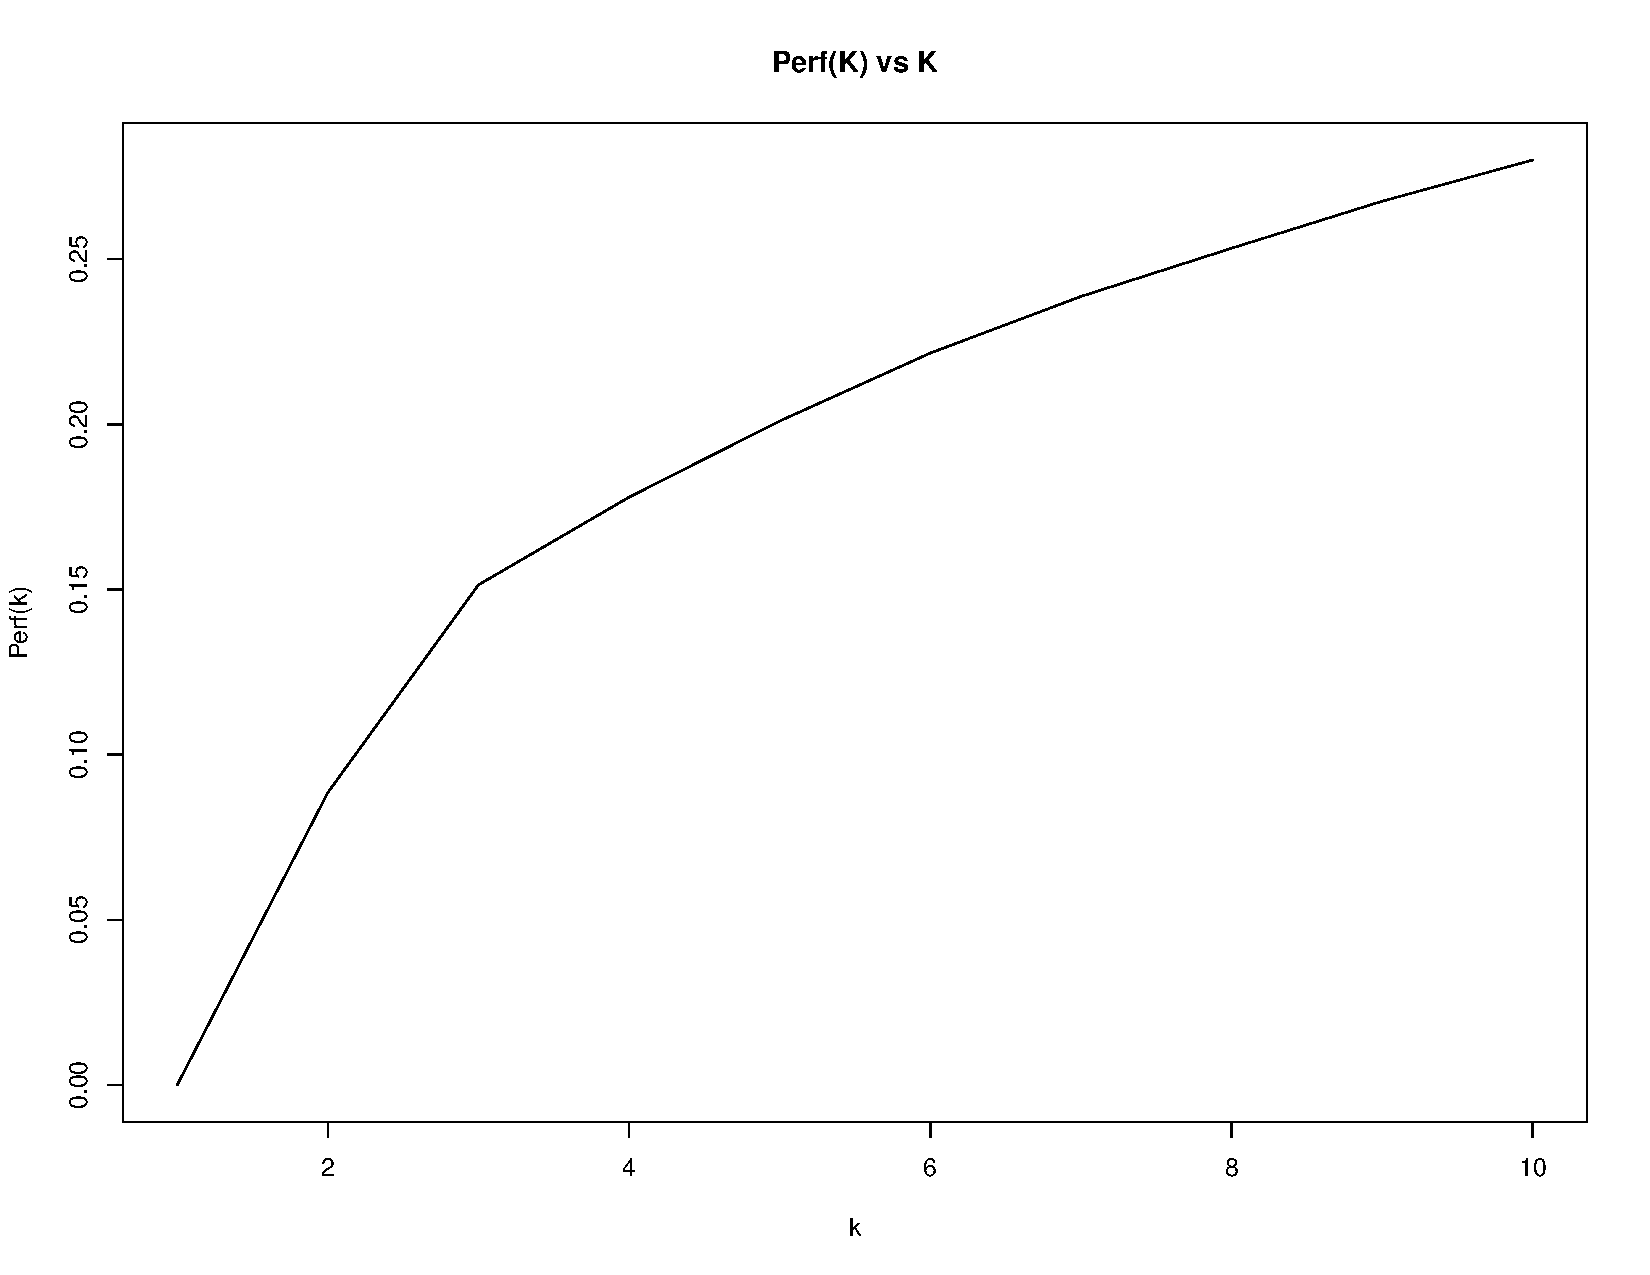
\includegraphics[width=12cm]{graphs/HW4_bestk1.pdf}
    \caption{Plot of Perf(K) vs K}
    \label{Perfk}
\end{figure}

The 'elbow' of perf(k) is at k=3, therefore three clusters is the optimal number. We verify this result by calculating and displaying the best k through the silhouette method, which measures the average distance between clusters. This can be seen in Figure \ref{Silh}. 

\begin{figure}[h]
    \centering
    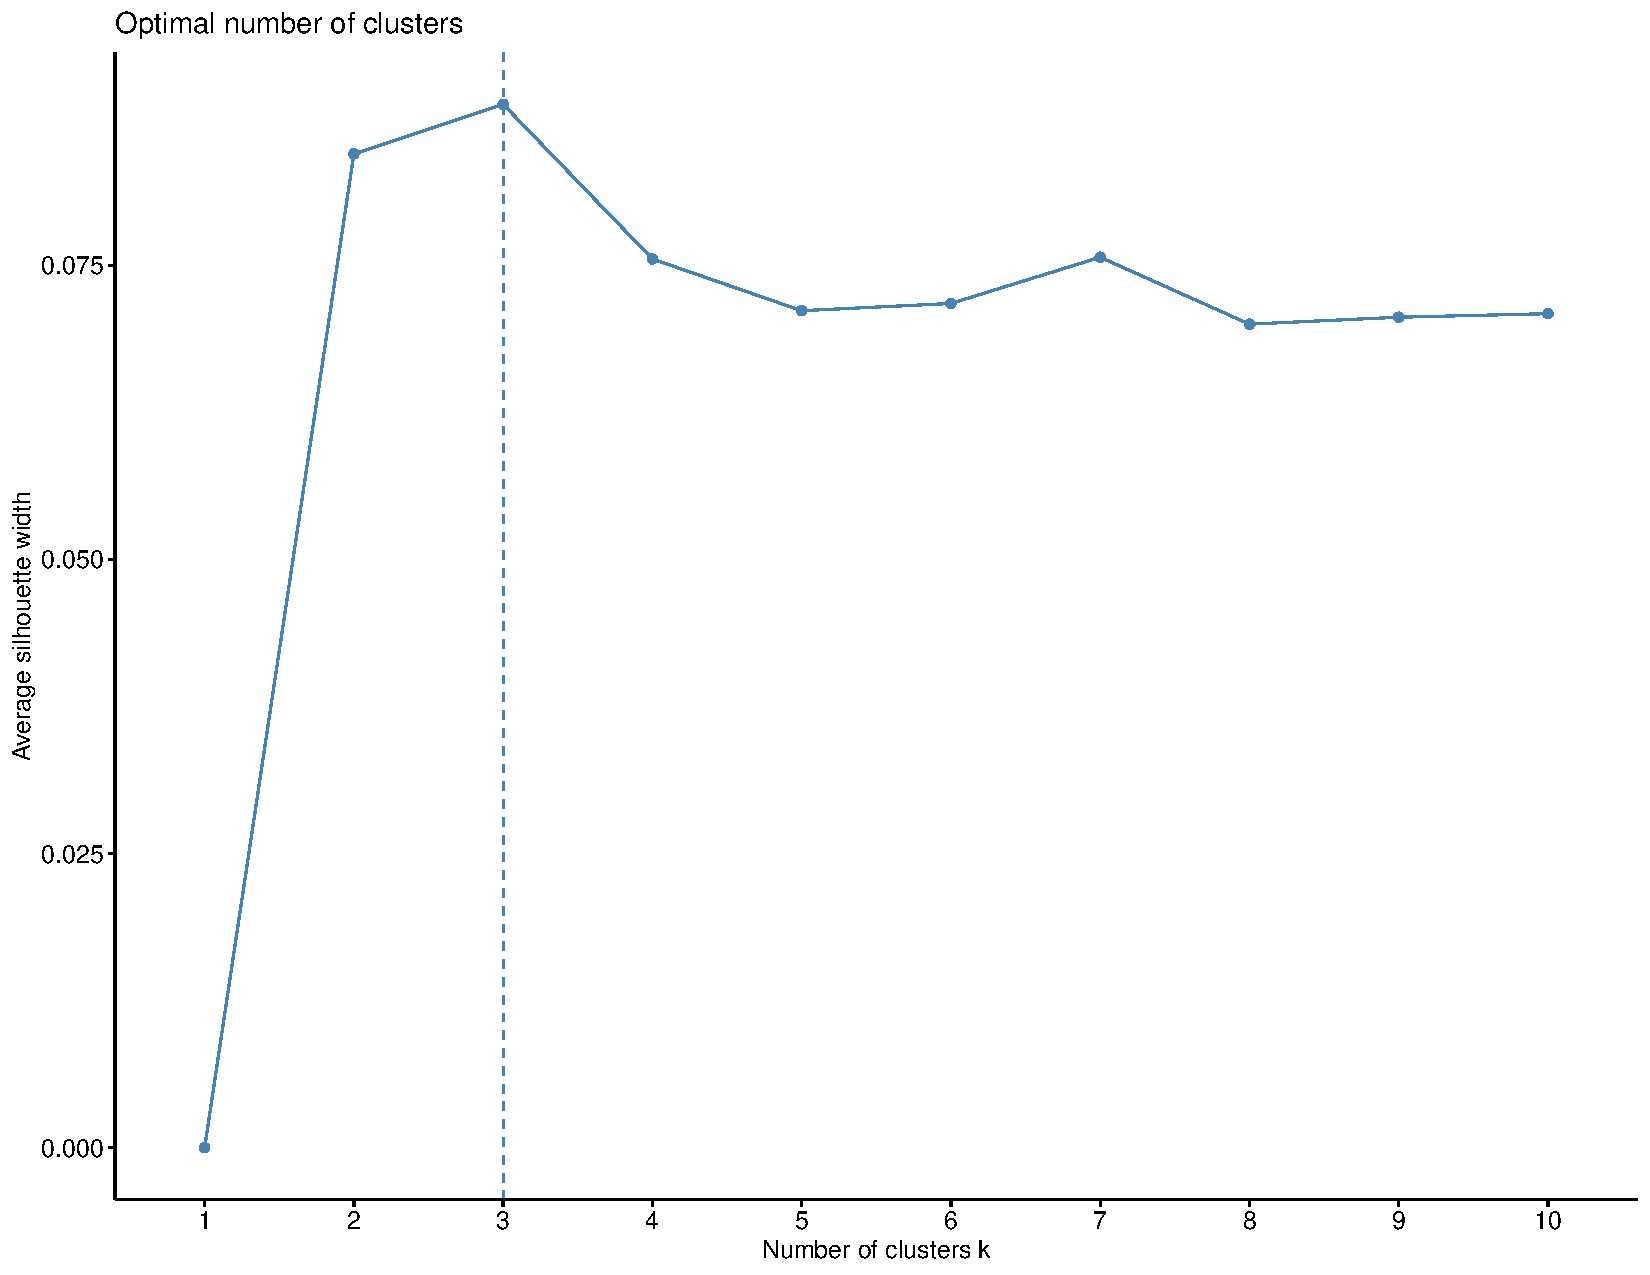
\includegraphics[width=12cm]{graphs/HW4_bestk.pdf}
    \caption{Selecting K through Silhouette Method}
    \label{Silh}
\end{figure}

This distance is maximized at k=3, further indicating that using three clusters is the best choice.

\newpage
\question % 2
We project the centers of each cluster into 3-dimensional space by utilizing their first three principal components. These projected centers are displayed in Table \ref{Proj} and visualized in Figure \ref{Cent}. 

\begin{table}[h]
    \centering
    {\begin{tabular}{c|ccc}
         &CLU1&CLU2&CLU3\\\hline
         x&5.99&13.93&0.00\\
         y&-17.45&-2.36&0.00\\
         z&11.45&-11.30&0.00
    \end{tabular}}\\
    \caption{Cluster Centers using Principal Components}
    \label{Proj}
\end{table}

\begin{figure}[H]
    \centering
    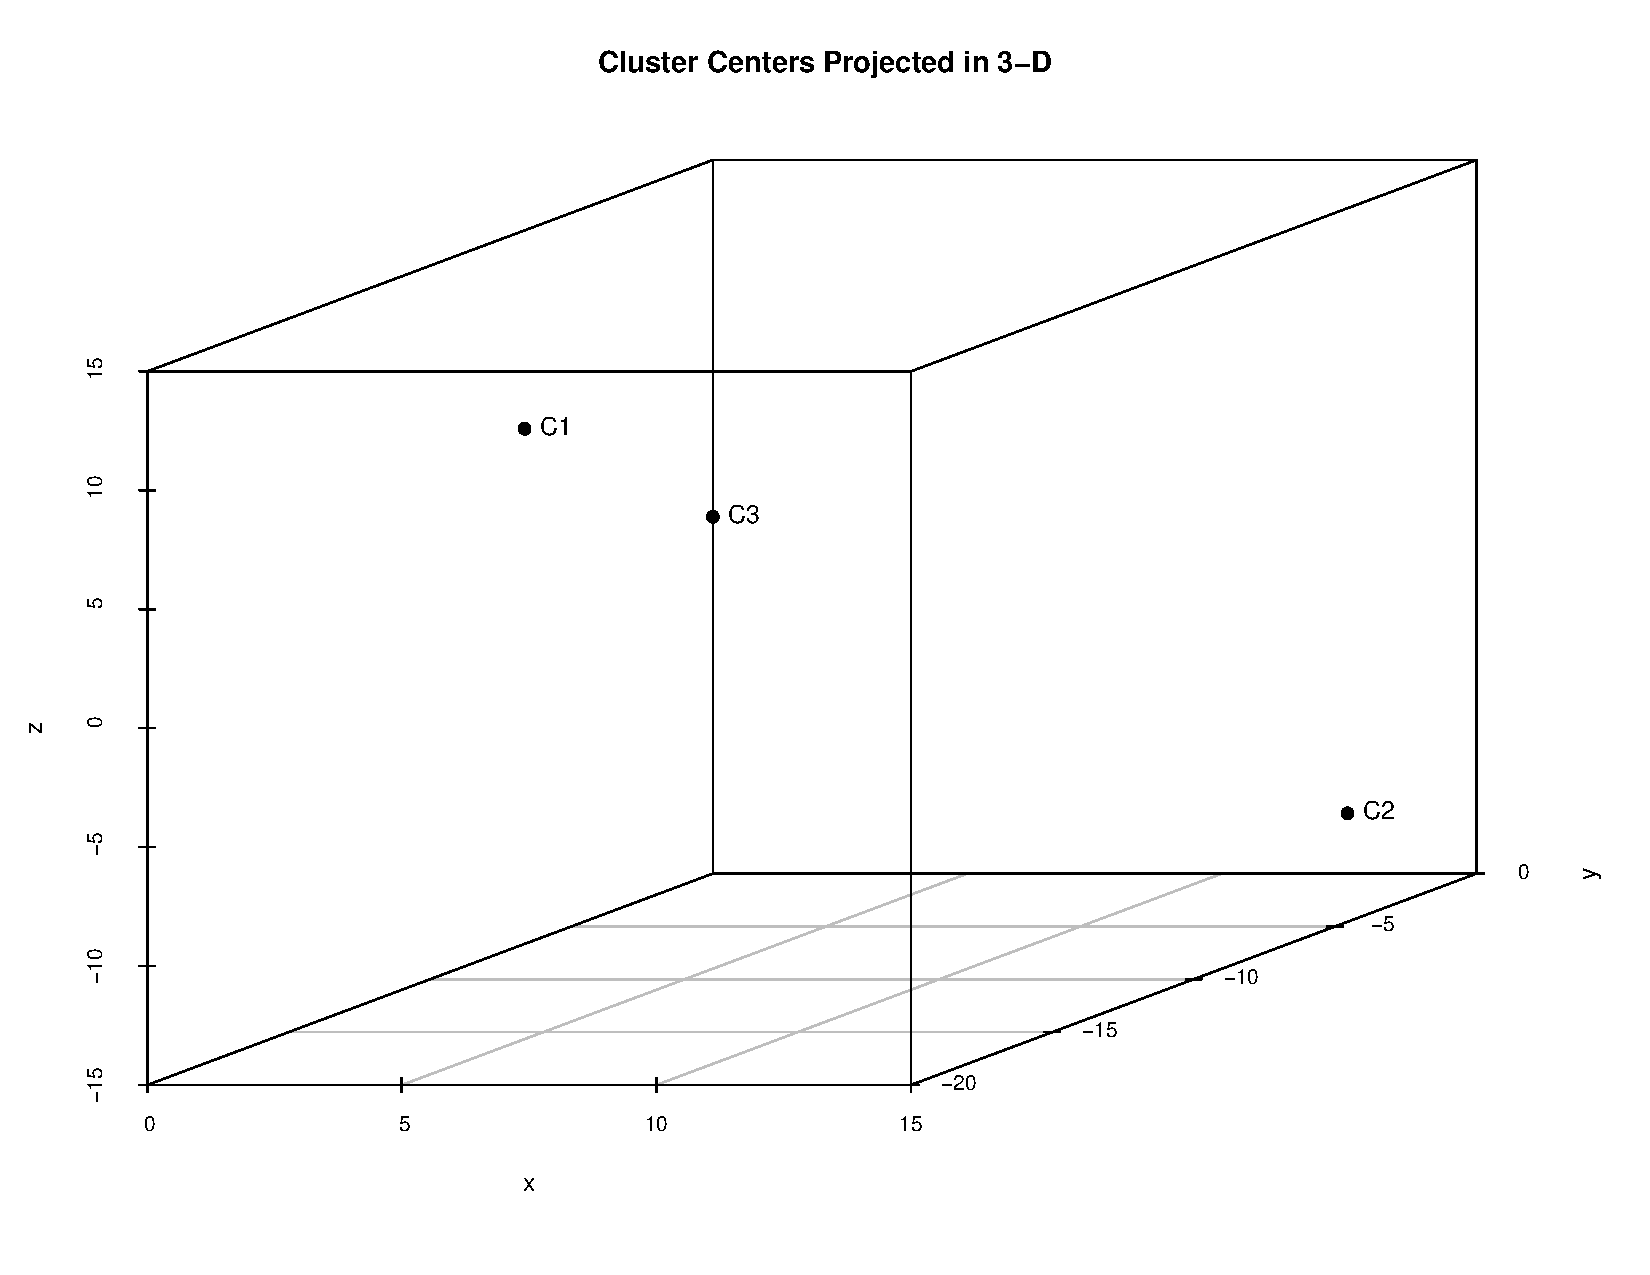
\includegraphics[width=12cm,height=8cm]{graphs/HW4_pcac.pdf}
    \caption{PCA Vectors C1, C2, C3}
    \label{Cent}
\end{figure}

Next, we took the cluster with the largest number of cases (cluster 2) and computed each case's 3-dimensional vector. These were then plotted as in Figure \ref{Pur}. 

\begin{figure}[H]
    \centering
    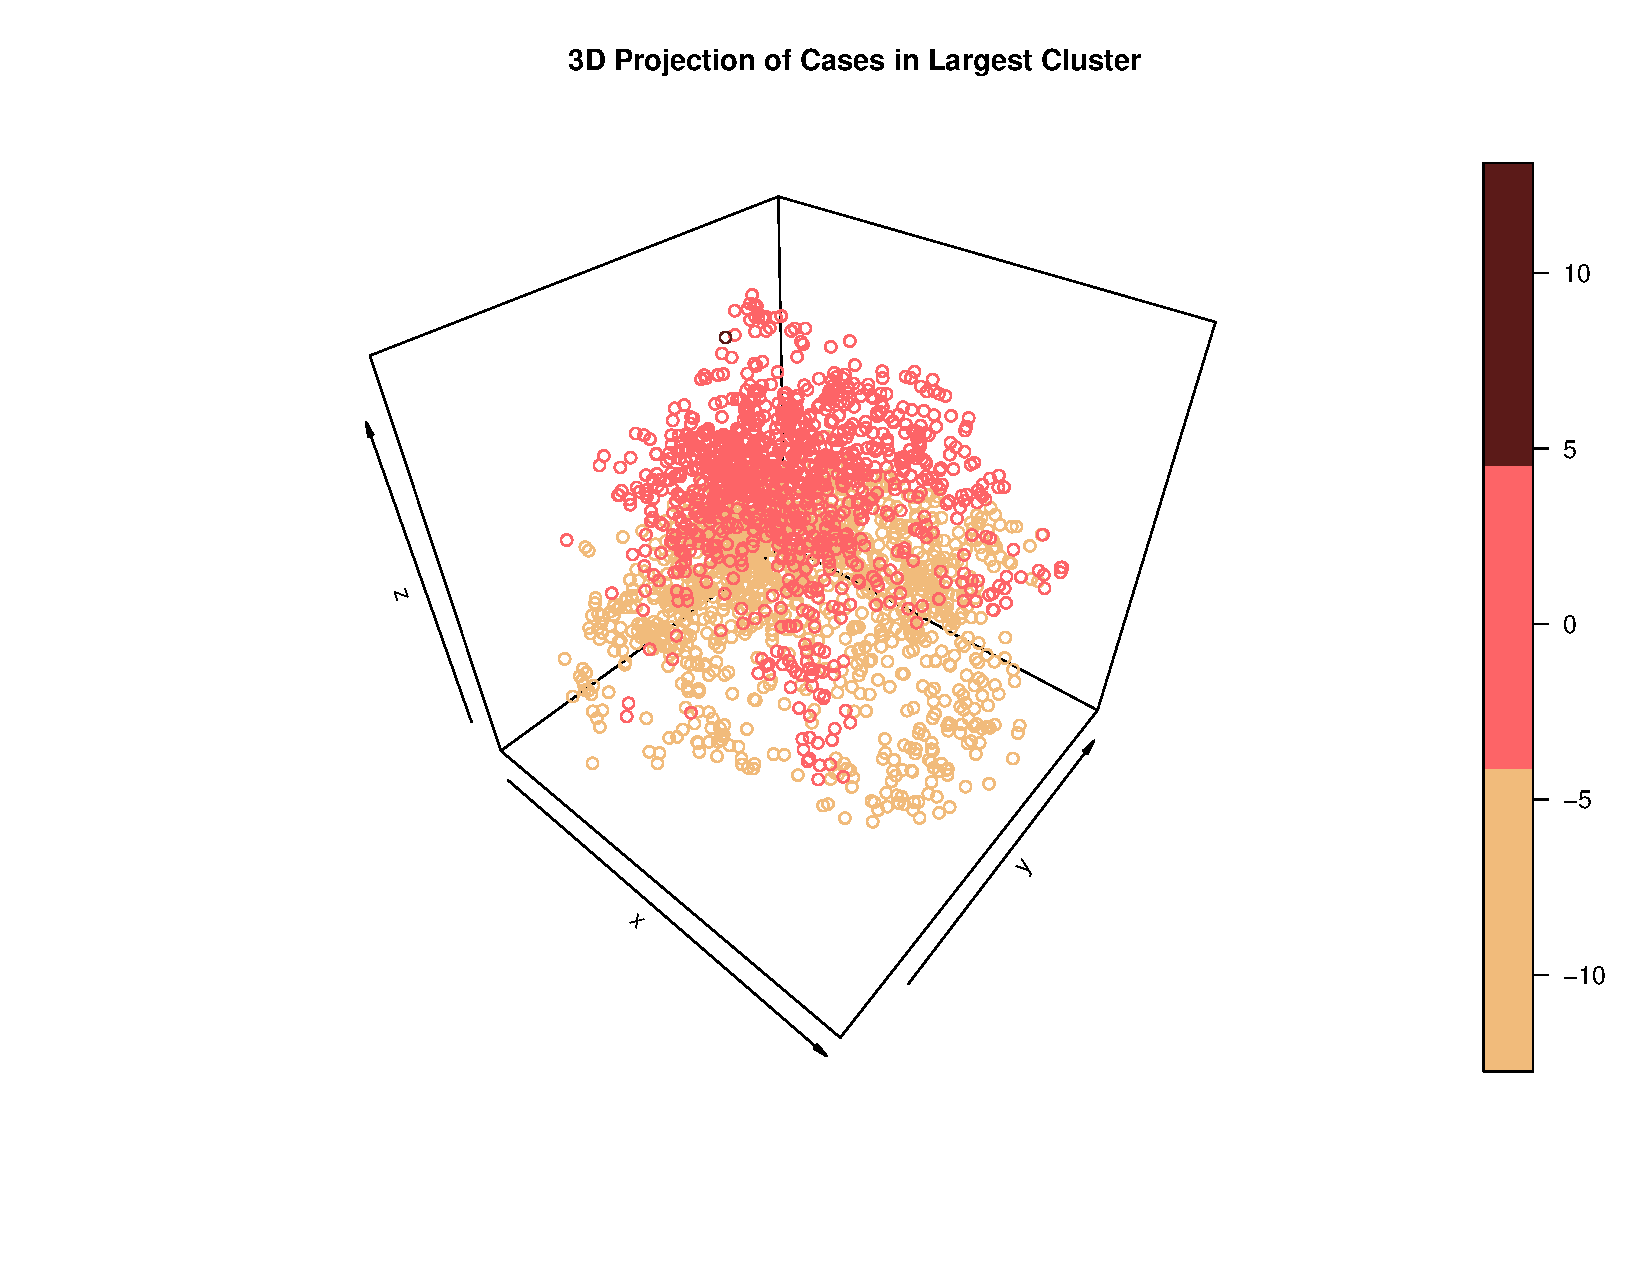
\includegraphics[width=12cm,height=8cm]{graphs/HW4_bigclu.pdf}
    \caption{Purity of Largest Cluster}
    \label{Pur}
\end{figure}

Figure \ref{Pur} shows that our largest cluster is not pure. In fact, all three classes are represented, though Bitstream (pink) and Consolas (beige) are the most prominent.

\question % 3
We computed the Gini coefficient for each cluster and summed them to reach the clustering's \textbf{total impurity, 1.602}. With three classes our maximum impurity is 2. Thus, the clustering exercise does not appear to be accurately separating the cases. Table \ref{Freq} shows the frequency of each class in the three clusters. Cluster 1 is approximately 15\% Bitstream, 54\% Consolas, and 31\% Ebrima.

\begin{table}[h]
    \centering
    {\begin{tabular}{c|ccc}
         &CLU1&CLU2&CLU3\\\hline
         Bitstream&0.15&0.78&0.24\\
         Consolas&0.54&0.16&0.36\\
         Ebrima&0.31&0.06&0.40
    \end{tabular}}\\
    \caption{Frequency of Class in Clusters}
    \label{Freq}
\end{table}

\question % 4
We then constructed a simple classifier based on the k-means clustering. The class that occurred most frequently in each cluster was used to classify the cases. For example, Cluster 1's most frequently occurring class was Consolas, so every case in Cluster 1 was predicted to be of class Consolas. Cluster 2's most frequently occurring class was Bitstream, and Cluster 3's was Ebrima. The confusion matrix for this method is displayed in Table \ref{Conf}.

\begin{table}[h]
    \centering
    {\begin{tabular}{c|ccc}
         &BITSTREAM&CONSOLAS&EBRIMA\\\hline
         BITSTREAM&0.60&0.14&0.26\\
         CONSOLAS&0.12&0.48&0.39\\
         EBRIMA&0.06&0.37&0.57
    \end{tabular}}\\
    \caption{Confusion Matrix for K-Means. True class along the row, Predicted class along the column}
    \label{Conf}
\end{table}

The k-means classifier has a \textbf{global accuracy of 55\%}. The diagonal of the confusion matrix provides useful information in relation to the frequency matrix. Specifically, the diagonal represents the total percentage of cases within the respective cluster of each class. Recall that Cluster 1's most frequently occurring class was Consolas. Table \ref{Freq} shows that Consolas comprised 54\% of Cluster 1. Examining the Consolas entry on the confusion matrix, we see that 48\% of its total cases were classified correctly. This implies that 48\% of Consolas's true total cases were in Cluster 1, and 52\% of its true total cases were outside Cluster 1.

\newpage
\lstinputlisting{code.R}
\end{document}
